\documentclass[main.tex]{subfiles}
\begin{document}
\bigskip

\subsection{Partitions, Young diagrams, and Littlewood-Richardson coefficients}
This thesis studies combinatorial aspects of injective tensor $\mathfrak{sp}_\infty-, \mathfrak{so}_\infty-$modules, and we start with some necessary background for understanding the Littlewood-Richardson rule for semistandard skew tableaux. In this section, we make use of \cite{fulton1991representation} and \cite{andrews1998theory} for the theory, and present it in a similar manner to the Bachelor's theses \cite{zokirovathesis} and \cite{weissthesis}.\\

\begin{defn}[\textbf{Partition}] 
A partition $\lambda$ of $n$ is a finite non-increasing sequence of positive integers $\lambda_1, \lambda_2, ..., \lambda_r$ such that $\sum\limits_{i=1}^{r}\lambda_r = n.$ We use the notation $\lambda = (\lambda_1, \lambda_2, ..., \lambda_r)$, and say that the $\lambda_i, $ for $i=\overline{1,r}$, are the parts of the partition $\lambda.$ 
\end{defn}

A useful way to compare partitions is by the \textbf{lexicographic order} (more details in \cite{wikipediaorder}). \\

\begin{defn}[\textbf{Lexicographic order on partitions}]
    Let $\lambda = (\lambda_1, \lambda_2, ...)$ and $\mu=(\mu_1, \mu_2, ...)$ be two partitions. We say that $\lambda$ precedes $\mu$ or $\mu$ succeeds $\lambda$ in the lexicographic order, and write $\lambda <_{lex} \mu$ or $\mu>_{lex}\lambda$,  if $\lambda \neq \mu$ and for the smallest $k$ where $\lambda_k\neq\mu_k$ we have $\lambda_k<\mu_k.$
\end{defn}
\bigskip

Each partition $\lambda$ can be represented graphically via a \textbf{Young diagram}. Such diagram consists of finitely many boxes, organized in succeeding rows. For $\lambda = (\lambda_1, \lambda_2, ..., \lambda_r),$ the  $i^{\text{th}}$ row has $\lambda_i$ boxes.\\
\begin{figure}[h]
    \centering
    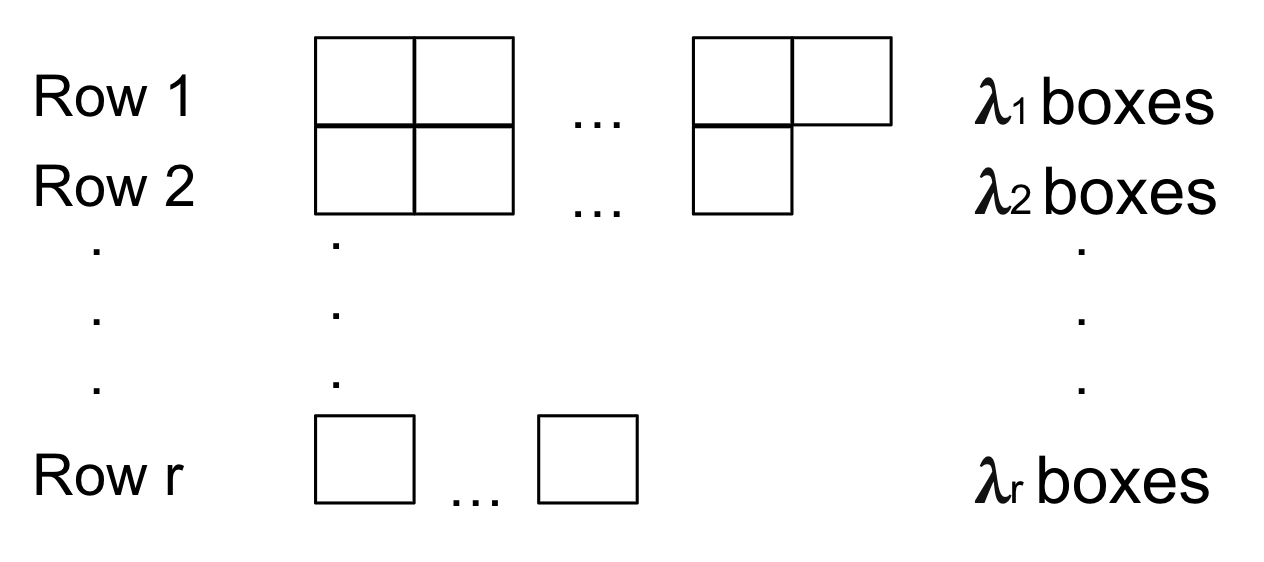
\includegraphics[width=0.4\linewidth]{images/GeneralYoungDiag.png}
    \caption{Young diagram of $\lambda = (\lambda_1, \lambda_2, ..., \lambda_r)$.}
    \label{fig:generalyoungdiag}
\end{figure}

\begin{ex}
\label{ex-youngdiagram}
    Let us look at $\lambda=(4,4,2,1)$ which is a partition of $11$. The Young diagram of $\lambda$ has two rows with 4 boxes, a row with 2 boxes, and a final row with 1 box. 
    \begin{figure}[h]
        \centering
        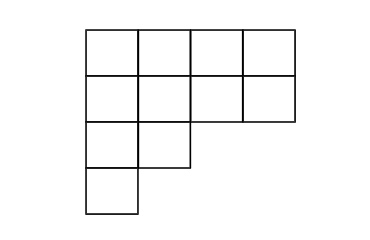
\includegraphics[width=0.25\linewidth]{images/YoungDiagram.png}
        \caption{Young diagram of the partition (4,4,2,1).}
        \label{fig:fig-youngdiagram}
    \end{figure}
\end{ex}

A \textbf{Young tableau} is a Young diagram with boxes filled with numbers from $1$ to \textbf{the degree of the partition} $|\lambda|:=\sum\limits_{i=1}^{r}\lambda_i$.\\
\bigskip

\begin{defn}[\textbf{Subpartition}]
    Let $\lambda=(\lambda_1, \lambda_2, ..., \lambda_r)$ be a partition. We say that a partition $\mu=(\mu_1, \mu_2, ..., \mu_s)$ is a \textbf{subpartition} of $\lambda$ if $s\leq r$ and $\mu_i\leq\lambda_i,$ for $1\leq i\leq s.$
\end{defn}

\textbf{Remark.} If $\mu$ is a subpartition of $\lambda$, then the Young diagram of $\mu$ is graphically included in the Young diagram of $\lambda$ so that the top left boxes of both diagrams coincide.

\begin{ex}
    \label{ex-subpartition}
    Let us draw the Young diagrams of $\lambda=(4,4,2,1)$ and $\mu=(4,2,1,1)$ (one of the subpartitions of $\lambda$) according to our graphical convention. The highlighted boxes are part of both Young diagrams.\\
    
    \begin{figure}[H]
        \centering
        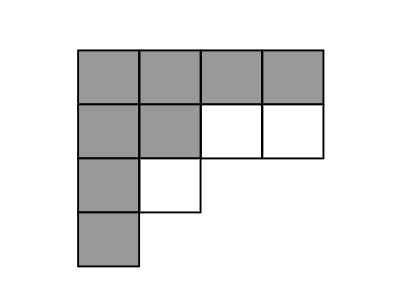
\includegraphics[width=0.25\linewidth]{images/Subpartition.png}
        \caption{The Young diagram of $(4,4,2,1)$ and the Young diagram of $(4,2,1,1)$ with highlighted boxes for emphasising the subpartition property.}
        \label{fig:subpartition}
        
    \end{figure}
    
\end{ex}

\bigskip

Given a Young diagram corresponding to partition $\lambda = (\lambda_1, \lambda_2, ..., \lambda_r)$, we can transpose it (reflect it by the main diagonal) to obtain the \textbf{transposed Young diagram} - this corresponds to the \textbf{conjugate partition} $\lambda^T$. Moreover, $|\lambda|=|\lambda^T|$ and 
    $$
    \lambda^T = (\;\underbrace{r, r, ..., r,}_\text{$\lambda_r$ times}\;\; \underbrace{r-1, r-1, ..., r-1}_\text{$\lambda_{r-1}-\lambda_r$ times}, ..., \underbrace{1, 1, ..., 1}_\text{$\lambda_1-\lambda_2$ times}). 
    $$
    
\begin{ex}
\label{ex-conjugate}
    Given $\lambda = (4,3,1,1,1),$ we draw its Young diagram and then transpose it as in the figure \ref{fig:fig-conjugatediagram}.
    
    \begin{figure}[h]
        \centering
        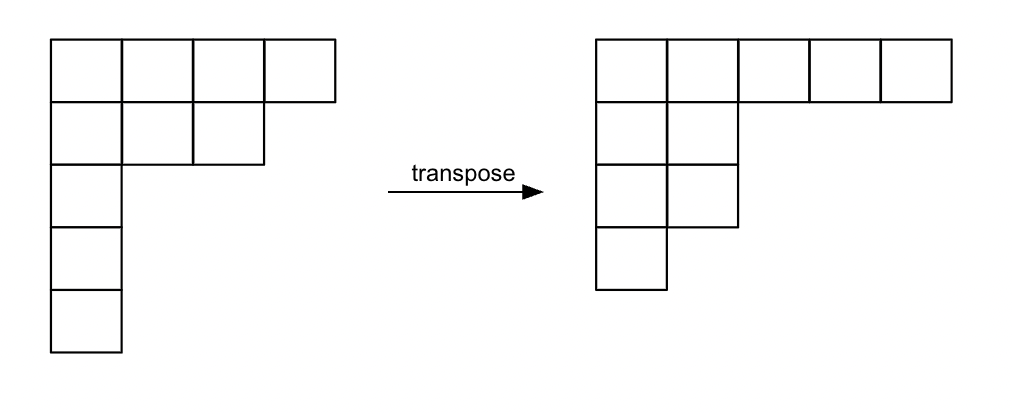
\includegraphics[width=0.5\linewidth]{images/ConjugateDiagram.png}
        \caption{The Young diagrams of the partition (4,3,1,1,1) and its conjugate }
        \label{fig:fig-conjugatediagram}
    \end{figure}
    
    The transposed diagram is the Young diagram of the partition $$\lambda^T = (5,2,2,1) 
    = (\;\underbrace{5}_\text{$\lambda_5=1$ time}\;\;, \underbrace{2, 2}_\text{$\lambda_{2}-\lambda_3=2$ times}, \underbrace{1}_\text{$\lambda_1-\lambda_2=1$ time}),$$
    and $|\lambda|=|\lambda^T| = 10.$ \\
\end{ex}  
\bigskip

Another operation we can do on partitions is \textbf{multiplication by a positive integer}. For $\lambda = (\lambda_1, \lambda_2, ..., \lambda_r)$ and some natural number $k,$ we define $k\lambda$ as the partition $(k\lambda_1, k\lambda_2, ..., k\lambda_n)$.
\bigskip

\begin{lemma}
    \label{lemma-double-conjugate}
    Given a partition $\lambda$ and its conjugate $\lambda^T$, the Young diagram of $(k\lambda)^T$ is obtained from the Young diagram of $\lambda^T$ by repeating each row of $\lambda^T$  $k$ times: if  $\lambda^T = ((\lambda^T)_1, (\lambda^T)_2, ..., (\lambda^T)_m),$ then $$(k\lambda)^T=(
    \underbrace{(\lambda^T)_1, (\lambda^T)_1, ..., (\lambda^T)_1}_\text{$k$ times},
    \underbrace{(\lambda^T)_2, (\lambda^T)_2, ..., (\lambda^T)_2}_\text{$k$ times}, ..., \underbrace{(\lambda^T)_m, )(\lambda^T)_m, ..., (\lambda^T)_m}_\text{$k$ times}).
    $$
\end{lemma}

\begin{proof}
   Straightforward.
\end{proof}
\bigskip

\begin{ex}
\label{ex-double-conjugate}
    Given $\lambda = (4,3,1,1,1),$ we have $2\lambda = (8,6,2,2,2).$ Hence, by computing the conjugate partitions, we obtain $\lambda^T = (5,2,2,1)$ and $2\lambda^T = (5,5,2,2,2,2,1,1)$. See figure \ref{fig:fig-double-conjugate}.\\
    
    \begin{figure}[H]
        \centering
        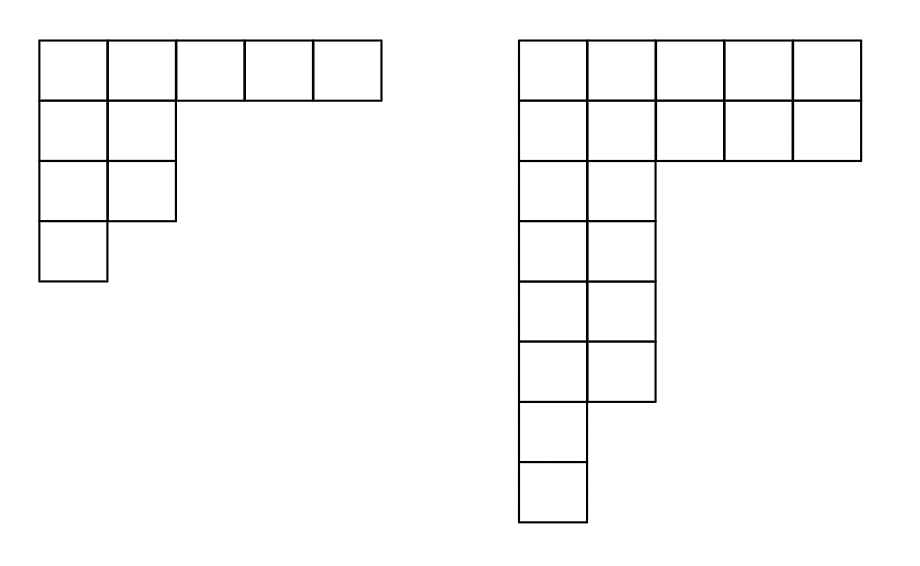
\includegraphics[width=0.5\linewidth]{images/DoubleTranspose.png}
        \caption{Young diagrams for $\lambda^T = (5,2,2,1)$ and $2\lambda^T = (5,5,2,2,2,2,1,1)$.}
        \label{fig:fig-double-conjugate}
    \end{figure}
\end{ex}
\bigskip

Next, we introduce some special types of partitions, which will be particularly useful in section 4 of this thesis when discussing injective resolutions of $\mathfrak{sp}_\infty-$modules. We define them according to the description in \cite{SAM_2015}, and give examples in figure \ref{fig:cqs-rqs-partitions}.

\begin{defn}[\textbf{Column-quasi-symmetric partitions. Row-quasi-symmetric partitions}]
\label{def-cqs}
    Let $\lambda$ be a partition. We say that $\lambda$ is a \textbf{column-quasi-symmetric (CQS)}  partition if for each box $b$ along the main diagonal of the Young diagram of $\lambda$, the number of boxes below $b$ in the same column minus 1 equals the number of boxes to the right of $b$ in the same row. \\
    In a similar manner, $\lambda$ is a \textbf{row-quasi-symmetric (RQS)}  partition if for each main diagonal box $b$, the number of boxes to the right of $b$ on the same row minus 1 equals the number of boxes below $b$ in the same column. 
\end{defn}

\begin{figure}[h]
    \centering
    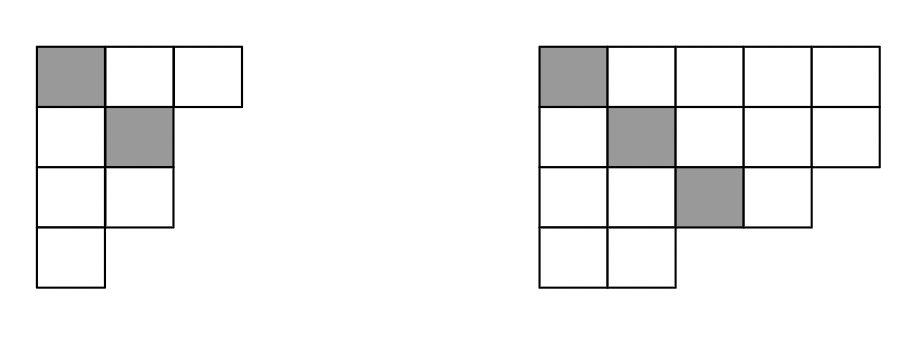
\includegraphics[width=0.5\linewidth]{images/CQS-RQS.png}
    \caption{Young diagrams for a CQS partition (left) and a RQS partition (right). The boxes on the main diagonal are highlighted.}
    \label{fig:cqs-rqs-partitions}
\end{figure}


Before introducing the Littlewood-Richardson rule, we introduce \textbf{Schur polynomials}. These form a basis of the vector space of homogeneous symmetric polynomials of degree $n$ in $k$ variables $x_1, x_2, ..., x_k$. The Schur polynomials are used in the theory of symmetric functions and in representation theory - more details can be found in \cite{fulton1991representation} (Appendix A, and chapter 1.4). However, we will focus on the fact that they are indexed by partitions, and will provide explanations and relevant examples to showcase the connection with Young diagrams. \\

\begin{defn}[\textbf{Schur polynomial}]
Let $\lambda=(\lambda_1, \lambda_2, ..., \lambda_r)$ be a partition of $n$. Fix a positive integer $k\geq n$ and set $\lambda_{r+1}=\lambda_{r+2}=...=\lambda_{k}=0.$ The \textbf{Schur polynomial} corresponding to $\lambda$ and in variables $x_1, x_2, ..., x_k$ is 
$$
S_\lambda^k = \frac{|((x_j^{\lambda_i+k-i})_{1\leq i,j \leq k})|}{\Delta},
$$
where $|((x_j^{\lambda_i+k-i})_{1\leq i,j \leq k})| = \text{det }$ 
$\begin{pmatrix}
    x_1^{\lambda_1+k-1} & x_2^{\lambda_1+k-1} & ... & x_k^{\lambda_1+k-1}\\
    x_1^{\lambda_2+k-2} & x_2^{\lambda_2+k-2} & ... & x_k^{\lambda_2+k-2}\\
    \vdots & \vdots & \ddots & \vdots \\
    x_1^{\lambda_k} & x_2^{\lambda_k} & ... & x_k^{\lambda_k}
\end{pmatrix} $
and $\Delta = \prod\limits_{1\leq i < j \leq k} (x_i-x_j).$ 
% = |((x_j^{r-i})_{1\leq i\leq r})|$.
\end{defn}
\textbf{Remark.} Note that $\text{deg}\;S_\lambda^k=n$.
\bigskip

\begin{ex}
    \label{ex-schur-polynomial}
    Let us look at the Schur polynomials of degree $2$ in $4$ variables $x_1, x_2, x_3, x_4$. The partition set we are interested in is $\{(2), (1,1)\}.$ Our Schur polynomials are:
    $$
    S_{(2)}^4 := x_1^2 + x_2^2 + x_3^2 + x_4^2 + x_1 x_2 + x_1 x_3 + x_1 x_4 +
    x_2 x_3 + x_2 x_4 + x_3 x_4,
    $$
    $$
    S_{(1,1)}^4 := x_1 x_2 + x_1 x_3 + x_1 x_4 + x_2 x_3 + x_2 x_4 + x_3 x_4.
    $$
\end{ex}
\bigskip

Next, we explain how the product of two Schur polynomials is expressed as a linear combination of Schur polynomials. First, we take a basic example of multiplying the polynomials above by $S_{(1)}^4$, and then we present the Pieri formula for multiplying a Schur polynomial with another Schur polynomial corresponding to a partition of length one (row-partition).
\bigskip

\begin{ex}
    \label{ex-schur-mult}
    We multiply the Schur polynomials of degree $2$ in $4$ variables (from example \ref{ex-schur-polynomial}) by the Schur polynomial of degree $1$ in $4$ variables $S_{(1)}^4 := x_1 + x_2 + x_3 + x_4$. The result is: 
    \bigskip
    $$
    S_{(2)}^4 \cdot S_{(1)}^4 = (x_1^3 + x_2^3 + x_3^3 + x_4^3) + 
    2(x_1^2 x_2 + x_1^2 x_3 + x_1^2 x_4 +
    x_2^2 x_1 + x_2^2 x_3 + x_2^2 x_4 + x_3^2 x_1 + x_3^2 x_2 + x_3^2 x_4 + x_4^2 x_1 + x_4^2 x_2 + x_4^2 x_3 + x_4^2 x_3) 
    $$
    $$
    + 3(x_1 x_2 x_3 + x_1 x_2 x_4 + x_1 x_3 x_4 + x_2 x_3 x_4) = S_{(3)}^4+S_{(2,1)}^4,
    $$
    $$
    S_{(1,1)}^4 \cdot S_{(1)}^4= 
    (x_1^2 x_2 + x_1^2 x_3 + x_1^2 x_4 + x_2^2 x_1 + x_2^2 x_3 + x_2^2 x_4 + x_3^2 x_1 + x_3^2 x_2 + x_3^2 x_4 + x_4^2 x_1 + x_4^2 x_2 + x_4^2 x_3) 
    $$
    
    $$
    + 3(x_1 x_2 x_3 + x_1 x_2 x_4 + x_1 x_3 x_4 + x_2 x_3 x_4) = S_{(2,1)}^4 + S_{(1,1,1)}^4.
    $$
\end{ex}
\bigskip

\begin{thm}[\textbf{Pieri's formula}]
    Let $\lambda=(\lambda_1, \lambda_2, ..., \lambda_r)$ be a partition, let $(m)$ be a row-partition, and let $k\geq |\lambda|$. Then, by multiplying the Schur polynomials in $k$ variables $S_\lambda^k$ and $S_{(m)}^k$ we obtain $$S_\lambda^k \cdot S_{(m)}^k = \sum\limits_\mu S_\mu^k,$$ where the sum is over all partitions $\mu$ of length $r$ and of length $r+1$ such that, respectively, $\mu_1 \geq \lambda_1 \geq \mu_2 \geq \lambda_2 \geq ... \geq \mu_r \geq \lambda_r$ or $ \mu_1 \geq \lambda_1 \geq \mu_2 \geq \lambda_2 \geq ... \geq \mu_r \geq \lambda_r\geq \mu_{r+1}$ and $|\mu| = |\lambda|+m.$
\end{thm}

Equivalently, the theorem shows how the Young diagrams of the resulting partitions $\mu$ are obtained by attaching the $m$ boxes from the Young diagram of $(m)$ to the Young diagram of $\lambda$ so that no two attached boxes are on the same column of the resulting Young diagrams. We will refer to this as \textbf{Pieri's rule on Young diagrams}.
\bigskip

\begin{ex}
\label{ex-pieri}
    Let $\lambda = (3,2,2,1)$. We want to attach the three boxes from the Young diagram of $(3)$ the Young diagram of $\lambda$. According to the Pieri formula,  
    $$ S_{(3,2,2,1)}^k\cdot S_{(3)}^k = S_{(6, 2, 2, 1)}^k + S_{(5, 3, 2, 1)}^k + S_{(5, 2, 2, 2)}^k + S_{(5, 2, 2, 1, 1)}^k + S_{(4, 3, 2, 2)}^k + S_{(4, 3, 2, 1, 1)}^k + S_{(4, 2, 2, 2, 1)}^k + S_{(3, 3, 2, 2, 1)}^k,$$ 
    which leads to the resulting set of partitions $\{(6, 2, 2, 1), (5, 3, 2, 1), (5, 2, 2, 2),
    (5, 2, 2, 1, 1), (4, 3, 2, 2), \\ (4, 3, 2, 1, 1), (4, 2, 2, 2, 1), (3, 3, 2, 2, 1)\}$. The resulting Young diagrams are the ones in figure \ref{fig:pieri-example}, where the attached boxes are highlighted.
    \begin{figure}[h]
        \centering
        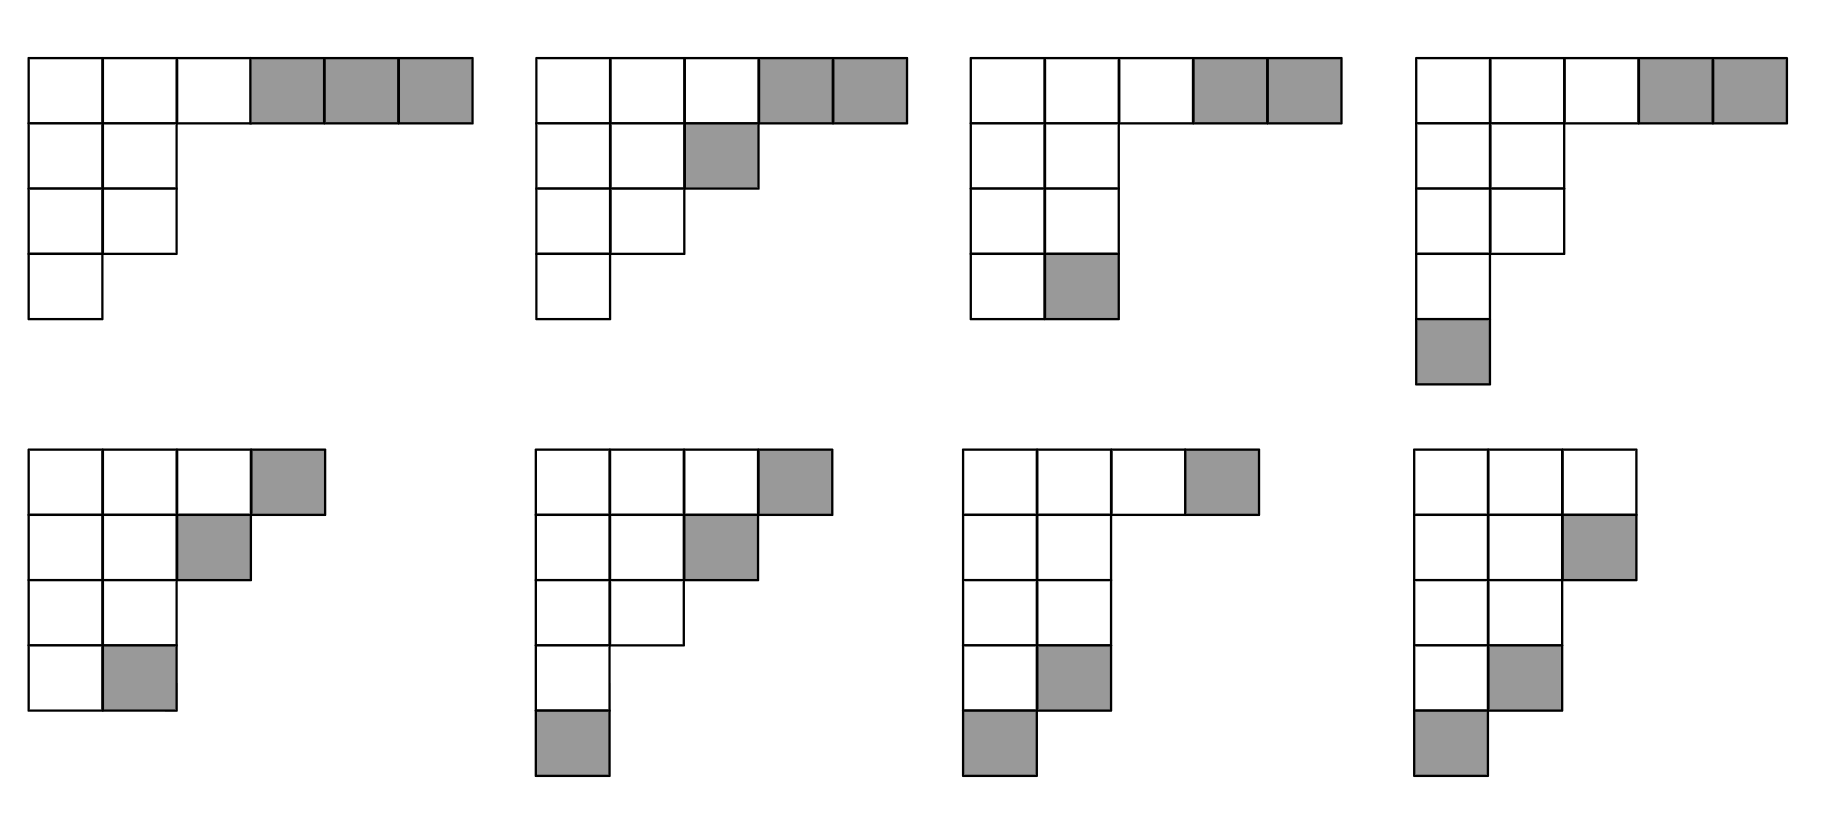
\includegraphics[width=0.75\linewidth]{images/PieriExample.png}
        \caption{}
        \label{fig:pieri-example}
    \end{figure}
\end{ex}

While Pieri's formula is a useful tool to multiply any Schur polynomial by a special Schur polynomial indexed by a row-partition, we need a generalized version for multiplying arbitrary Schur polynomials.
We can express the product as a linear combination of Schur polynomials with coefficients $\LR{\mu}{\lambda}{\gamma},$ as follows:

\begin{equation}
    \label{eq-LR-coeff-schur}
    S_\lambda^k \cdot S_\gamma^k = \sum_{\mu} \LR{\mu}{\lambda}{\gamma}S_\mu^k.
\end{equation}

\textbf{Remark.} When $\gamma$ is a row-partition, then $\LR{\mu}{\lambda}{\gamma} = \LR{\mu}{\gamma}{\lambda}$ equal either $0$ or $1$.\\

The coefficients $\LR{\mu}{\lambda}{\gamma}$ are called \textbf{Littlewood-Richardson coefficients} and they can be computed either from the expansion of the product of Schur polynomials, or with a combinatorial method involving Young diagrams (\cite{fulton1991representation} Appendix A). The combinatorial definition of the partitions $\mu$ which appear in the right-hand-side of the expression (\ref{eq-LR-coeff-schur}), is as follows:

\bigskip

\begin{defn}[\textbf{$\mathbf{\lambda-}$expansion of a Young diagram}]
    \label{def-partition-expansion}
    Let $\lambda = (\lambda_1, \lambda_2, ..., \lambda_r)$ be a partition considered as a Young diagram. A \textbf{$\lambda-$expansion} is a Young diagram (or a partition) $\mu$ partially filled with numbers, obtained by following the steps:
        \begin{itemize}
            \item add $\lambda_1$ boxes to the Young diagram of $\mu$ according to Pieri's rule, and write number $1$ in these boxes;
            \item add $\lambda_2$ boxes to the Young diagram obtained in the previous step, following Pieri's rule. Then write $2$ in those boxes;
            \item continue until the final $\lambda_r$ boxes filled with number $r$ are added to the Young diagram, according to Pieri's rule.
        \end{itemize}
    Let $t$ be any number in $\{1,2,...,|\lambda|\}$. We say that the expansion is \textbf{strict} if, among the first $t$ entries from right to left, and from the top row to the last row, each integer $k$ between $1$ and $r-1$ appears at least as many times as the number $k+1$.
\end{defn}

\bigskip

\begin{ex}
    \label{ex-partition-expansion}
    
    In this example, we will look at all strict $(2,1)-$expansions of the partition $(4,3)$. They appear in the right-hand-side of the following product of Schur polynomials:
    $$S_{(4,3)}^k \cdot S_{(2,1)}^k = S_{(6, 4)}^k + S_{(6, 3, 1)}^k + S_{(5, 5)}^k + 2S_{(5, 4, 1)}^k + S_{(5, 3, 2)}^k + S_{(5, 3, 1, 1)}^k + S_{(4, 4, 2)}^k + S_{(4, 4, 1, 1)}^k + S_{(4, 3, 2, 1)}^k .$$
    In terms of expansions of Young diagrams, we obtain the same results, as all possible strict $(2,1)-$expansions of $(4,3)$ are in figure \ref{fig:expansion-example}.
    \begin{figure}[H]
        \centering
        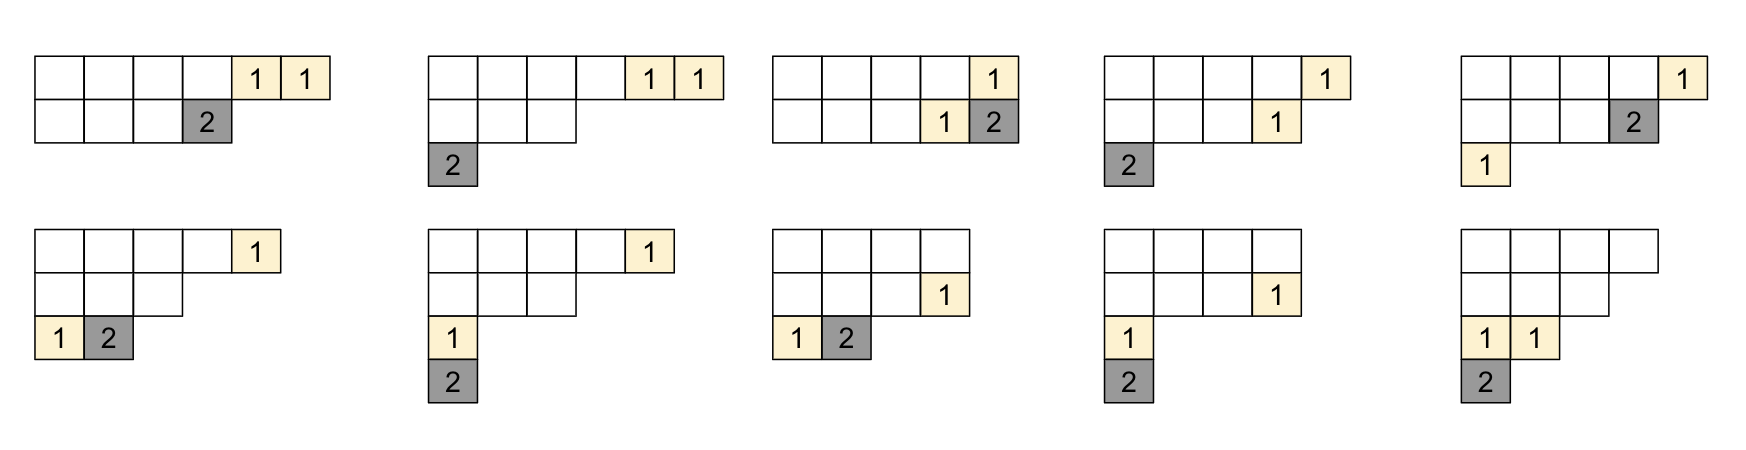
\includegraphics[width=0.9\linewidth]{images/ExpansionExample.png}
        \caption{The strict $(2,1)-$expansions of $(4,3)$. The 2 boxes with number 1 highlighted in yellow, and the box with number 2 in grey, for emphasis of the Pieri rule.}
        \label{fig:expansion-example}
    \end{figure}
    
\end{ex}
\bigskip

\begin{thm}[\textbf{Littlewood-Richardson combinatorial rule}, \cite{fulton1991representation}]
    Given three partitions $\mu, \lambda, \gamma$, the Littlewood-Richardson coefficients $\LR{\;\mu}{\lambda}{\gamma}$ represent the number of ways the Young diagram for $\mu$ can be obtained by a strict $\gamma-$expansion of the Young diagram of $\lambda.$
\end{thm}

 We notice that the theorem helps us find all partitions $\mu$ that can be obtained by attaching $\gamma$ to $\lambda$ - these are all partitions with nonzero Littlewood-Richardson coefficient, i.e. with $\LR{\;\mu}{\lambda}{\gamma}\neq 0.$ However, we can state the Littlewood-Richardson combinatorial rule in another manner, too. For this, we follow the outline presented in the Bachelor's theses \cite{zokirovathesis} and \cite{weissthesis}.\\
 
 Let $\lambda$ be a partition and $\mu$ be an expansion. We can look at the set-theoretic difference of these Young diagrams. The remaining skeleton of boxes is called a \textbf{skew diagram} of shape $\mu/\lambda$. 
\bigskip

 \begin{defn}[\textbf{Semistandard skew tableau}]
    \label{def-skew-tableau}
     Let $\lambda, \gamma, \mu$ be partitions such that $\lambda$ is a subpartition of $\mu$ and $|\gamma|=|\mu|-|\lambda|.$ A \textbf{semistandard skew tableau} of shape $\mu/\lambda$ and weight $\gamma$ is a skew diagram filled with numbers such that:
     \begin{itemize}
         \item each positive integer $k\leq|\gamma|$ occurs exactly $\gamma_k$ times,
         \item each column's entries are strictly increasing (left to right),
         \item each row's entries are weakly increasing (top to bottom row).
     \end{itemize}
     Moreover, if after removal of one or more leftmost column we still have a semistandard skew tableau, then our semistandard skew tableau of shape $\mu/\lambda$ and weight $\gamma$ is called a \textbf{Littlewood-Richardson tableau.}
 \end{defn}

 \bigskip



 Then, all partitions $\gamma$ for which $\LR{\;\mu}{\lambda}{\gamma}\neq 0$ can be found through Littlewood-Richardson tableaux. Additionally, we can rephrase the combinatorial rule as follows:

\bigskip

 \begin{thm}[\textbf{Littlewood-Richardson combinatorial rule}, \cite{wikipedialittlewoodrichardson}]
 \label{LR-comb-rule-tableaux}
     Given three partitions $\mu, \lambda, \gamma$, the Littlewood-Richardson coefficient $\LR{\;\mu}{\lambda}{\gamma}$ is equal to the number of Littlewood-Richardson tableaux of shape $\mu/\lambda$ and weight $\gamma$.
 \end{thm}
\bigskip

\begin{crl}
    \label{crl-expansion-tableau}
     The conditions for a strict $\gamma-$expansion of a Young diagram of $\lambda$ to the Young diagram of $\mu$ are equivalent to the conditions in the definition of a Littlewood-Richardson tableau of shape $\mu/\lambda$ and weight $\gamma$.
\end{crl}

% PART 2  
\subsection{Modules and socle filtrations of modules}

In order to introduce the notions of socle filtrations, we need to discuss some algebraic background. We will follow the structure of the early preliminaries sections in \cite{zokirovathesis} and \cite{weissthesis}.\\

\begin{defn}[\textbf{Module over a Lie algebra}]
Let $\mathfrak{g}$ be a Lie algebra. A $\mathfrak{g}-$module M is a vector space equipped with a bilinear map $\mathfrak{g}\times M\to M, (x,m)\mapsto x\cdot m$ satisfying 
$$[x,y]\cdot m = x\cdot (y\cdot m) - y\cdot (x\cdot m), \;\;\; \forall x,y\in\mathfrak{g}, \forall m\in M.$$    
\end{defn}

\bigskip

Let us take an $R$-module $M$, where $R$ is a ring or a Lie algebra. 

\begin{defn}[\textbf{Simple module. Semisimple module}]
    Let $M$ be a nonzero $R-$module. We say that $M$ is a \textbf{simple module} if it does not have any proper submodules. \\
    
    We call $M$ a \textbf{semisimple} module if one of the following equivalent conditions is satisfied:
    \begin{itemize}
        \item $M$ is a direct sum of simple submodules, or
        \item $M$ is the sum of all its simple submodules, or
        \item Any submodule $M_0\subset M$ admits a direct complement $M_1\subset M$ (i.e. $M = M_0\oplus M_1$).
    \end{itemize}
\end{defn}

\bigskip

The equivalence of the conditions in the definition above is proven in \cite{lang2012algebra} (chapter XVII).\\


\begin{defn}[\textbf{Indecomposable modules. Decomposable modules}]
    Let $M$ be a nonzero $R-$module. If $M$ cannot be written as a direct sum of two nonzero submodules, then it is called \textbf{indecomposable.} Otherwise, it is \textbf{decomposable.}
\end{defn}

\bigskip

\begin{defn}[\textbf{Filtration of a module}]
Let $M$ be an $R-$module. A \textbf{ filtration} of module $M$ is a sequence of nested submodules of $M$
$$...\subset M_{i-1} \subset M_i \subset M_{i+1}\subset ... .$$

If the filtration is \textbf{strict}, i.e. if $M_{i-1}\neq M_i,$ for all $i,$ then the number of indices is the \textbf{length} of the filtration.
\end{defn}

\bigskip

For the rest of this section, we will be concerned about a particular type of filtration: the \textbf{socle} filtration. We will use the theory and notation in \cite{penkov2007tensorrepresentationsclassicallocally} for these concepts.
\bigskip

\begin{defn}[\textbf{Socle of a module}]
    We call the maximal semisimple submodule of an $R$-module \textbf{M} the \textbf{socle} of M, and write $\mathbf{soc\;M}$. By the above equivalence condition, the socle of $M$ is equal to the sum of all simple submodules of $M.$
\end{defn}

\begin{defn}[\textbf{Socle filtration}]
    We define the \textbf{socle filtration} of module $M$ inductively, as follows:
    \begin{itemize}
        \item $soc^{(1)}M = soc\;M,$
        \item For $i\geq 2,$ $soc^{(i)}M = p^{-1}(soc(M/ soc^{(i-1)}M)),$ where $p$ is the natural projection.
        % and where $soc^{(i)}M = soc^{(i-1)}M$ in case $soc(M/ soc^{(i-1)}M)$ does not exist.
    \end{itemize}
    % If the strict socle filtration is finite, the \textbf{length} of the socle filtration is given by the smallest integer $n$ such that $soc^{(n)}M=M$.\\
    We say that the socle filtration of $M$ is \textbf{exhaustive} if $\bigcup_i soc^{(i)}M = M.$

\end{defn}

\textbf{Remark.} Note that soc $M$ does not need to exist. (e.g. $\mathbb{C}[x]$ as a $\mathbb{C}[x]-$module does not have any simple submodules, hence its socle does not exist.) 

\bigskip
\begin{defn}[\textbf{Socle layers}]
Let $M$ be an $R-$module with finite and exhaustive socle filtration
 $$soc^{(1)}M \subset ... \subset soc^{(n)}M = M. $$ 
 We call the quotients of consecutive terms \textbf{socle layers}. They are denoted by $$\soc{i}M = soc^{(i)}M / soc^{(i-1)}M.$$
\end{defn}
\bigskip

\begin{ex}
\label{ex-socle-filtration}
    Let $A$ be an arbitrary but fixed $n\times n$ matrix such that its Jordan normal form has Jordan blocks only of size $k$. Let $\mathbb{C}[x]$ act on $\mathbb{C}^n$ by left multiplication with A:
    $$x
    \cdot 
    \begin{pmatrix}
        v_1 \\
        v_2 \\
        \vdots \\
        v_n
    \end{pmatrix}
    \mapsto 
    A
    \begin{pmatrix}
        v_1 \\
        v_2 \\
        \vdots \\
        v_n
    \end{pmatrix}
    $$
    Let us compute the socle filtration of $\mathbb{C}^n.$ First, we denote the eigenvalue corresponding to the $i$-th Jordan block by $\lambda_i$, where $1\leq i\leq \frac{n}{k}=:m$. We notice that each eigenspace will be a semisimple submodule, and that the eigenspace $ker(A-\lambda_iI)$ is spanned by one or more linearly independent eigenvectors of $\lambda_i$.
    Hence, using the inductive construction and denoting by $\mathbb{C}_\lambda$ the copy of $\mathbb{C}$ corresponding to eigenvalue $\lambda$, we obtain:
    $$soc^{(1)}\mathbb{C}^n = \mathbb{C}_{\lambda_1}\oplus \mathbb{C}_{\lambda_2}\oplus ... \oplus\mathbb{C}_{\lambda_m}, $$
    $$soc^{(2)}\mathbb{C}^n = \mathbb{C}_{\lambda_1}^2\oplus \mathbb{C}^2_{\lambda_2}\oplus ... \oplus\mathbb{C}^2_{\lambda_m}, $$
    $$\vdots$$
    $$soc^{(k)}\mathbb{C}^n = \mathbb{C}_{\lambda_1}^k\oplus \mathbb{C}^k_{\lambda_2}\oplus ... \oplus\mathbb{C}^k_{\lambda_m} = \mathbb{C}^n. $$
    The socle layers will be $$\soc{i}\mathbb{C}^n = soc^{(i)}\mathbb{C}^n / soc^{(i-1)}\mathbb{C}^n = \mathbb{C}_{\lambda_1}\oplus \mathbb{C}_{\lambda_2}\oplus ... \oplus\mathbb{C}_{\lambda_m},$$
    and we can represent all of them in the following table:
    \begin{table}[h]
        \centering
        \begin{tabular}{|c|}
            \hline
            $\mathbb{C}_{\lambda_1}\oplus \mathbb{C}_{\lambda_2}\oplus ... \oplus\mathbb{C}_{\lambda_m}$ \\
            \hline \vdots \\
           \hline $\mathbb{C}_{\lambda_1}\oplus \mathbb{C}_{\lambda_2}\oplus ... \oplus\mathbb{C}_{\lambda_m}$ \\
            \hline $\mathbb{C}_{\lambda_1}\oplus \mathbb{C}_{\lambda_2}\oplus ... \oplus\mathbb{C}_{\lambda_m}$ \\
            \hline
        \end{tabular} .
    \end{table}
\end{ex}
\bigskip

% INJECTIVE RESOLUTIONS
\subsection{Injective resolutions}
Next, we present some concepts from homological algebra that will be used in section 4 of the thesis. As reference we use \cite{weibel1994introduction}, \cite{phamthesis}, and \cite{wikipediainjectivemodule}. \\

Let $\mathcal{C}$ be a full subcategory of the category of left $R-$modules, where $R$ is a ring or a Lie algebra. All modules in this section are assumed to be objects of $\mathcal{C}.$
%injective module
\begin{defn}[\textbf{Injective object in a category of modules}]
A module $M$ in $\mathcal{C}$ is injective in $\mathcal{C}$ if it satisfies one of the following equivalent conditions:
\begin{itemize}
    \item if $M$ is a submodule of the left $R-$module $N,$ then there exists a submodule $P$ of $N$ such that $M\oplus P=N$
    \item any short exact sequence 
    $0\to M \to N \to P \to 0$
    of left $R-$modules splits
    \item If $X, Y$ are left $R$-modules, $f: X\to Y$ is an injective module homomorphism and $g:X\to M$ is an arbitrary module homomorphism, then there exists a module homomorphism $h:Y\to M$ such that the following diagram commutes:
    $$
        \begin{tikzcd}
            0 \arrow{r}{}
            & X \arrow{r}{f} \arrow{d}{g}
            & Y \arrow{ld}{h}
            \\
            & M  
        \end{tikzcd}
    $$
    \item $Hom(-, M)$, is an exact contravariant functor from the category of left $R$-modules to the category of abelian groups.
\end{itemize}
\end{defn}
% injective hull
\bigskip
\begin{defn}[\textbf{Injective hull}]
    An injective hull of an $R-$module $M$ is a minimal injective module containing $M.$
\end{defn}
\bigskip
%injective resolution 
\begin{defn}[\textbf{Right resolution. Injective resolution}]
    Let $M$ be a left $R-$module. A \textbf{right resolution} of $M$ is an exact sequence of $R-$modules
    $$0\to M \to I^1\to I^2 \to ... \to I^n \to ...$$
    The resolution is called \textbf{injective} if each $I^j$ is an injective $R-$module.
\end{defn}

 Note that if each $I^j$ in the injective resolution is the injective hull of the cokernel of the previous map, then we say that the injective resolution is \textbf{minimal}.\\

 Injective resolutions help us define the derived functor $Ext.$

 \begin{defn}[\textbf{Ext groups}]
 Let $B$ be a left $R-$module. For an injective resolution
 $$0\to B \to I^0\to I^1 \to ... \to I^n \to ...,$$
 there exists a corresponding complex
 $$
 \begin{tikzcd}
     0 \arrow{r}{h_0} &
     Hom_R(A, I^0) \arrow{r}{h_1}&  
     Hom_R(A, I^1) \arrow{r}{h_2}& ... ,
 \end{tikzcd}
 $$
 where $A$ is an $R-$module.
 For $i\geq 0$, the $i^{th}$ \textbf{Ext-group} $ Ext_\mathcal{C}^i(A,B),$ is the $i^{th}$ homology of this complex, i.e.
 $$
 Ext_\mathcal{C}^i(A,B) := ker(h^i) / im(h^{i-1}).
 $$     
 \end{defn}
 \bigskip
 \begin{prop}
     The $ Ext_\mathcal{C}^i(A,B)$ groups do not depend (up to isomorphism) on the choice of injective resolution of $B$.
 \end{prop}
\bigskip



% PART 3 
\subsection{Tensor representations of $\mathfrak{gl}_\infty,$ $\mathfrak{sp}_\infty,$ and $\mathfrak{so}_\infty$}

Next, we introduce the necessary background to understand the tensor representations of the classical locally finite Lie algebra $\mathfrak{gl}_\infty, \mathfrak{sp}_\infty,\text{ and } \mathfrak{so}_\infty$. More details can be found in \cite{penkov2007tensorrepresentationsclassicallocally} and \cite{dancohen2012koszulcategoryrepresentationsfinitary}. \\
\bigskip

Let $V, V_*$ be countable dimensional $\mathbb{C}-$vector spaces, and let $<\cdot, \cdot>:V\otimes V_{*}\to \mathbb{C}$ be a non-degenarate pairing. Then, the Lie algebra $\mathfrak{gl}_\infty$ is defined as the vector space $V\otimes V_{*}$ equipped with the Lie bracket
$$[u\otimes u^*, v\otimes v^*] = <u^{*}, v>u\otimes v^{*} - <v^{*},u>v\otimes u^{*}, \;\;\;\;\;\; u,v\in V, u^{*}, v^{*}\in V_{*},$$
and the Lie subalgebra $\mathfrak{sl}_\infty$ of $\mathfrak{gl}_\infty$ is defined as the kernel of the map $<\cdot,\cdot>$.
We can also provide a coordinate definition of $\mathfrak{gl}_\infty$ by giving its linear basis. It is shown in \cite{Mackey} that we can find dual bases $\{\xi_i\}_{i\in\mathfrak{J}}$ and $\{\xi_i^*\}_{i\in\mathfrak{J}}$ of $V$ and $V_*,$ respectively, indexed by $\mathfrak{J}$ countable, and such that $<\xi_j^*, \xi_i> = \delta_{i,j},$ for $i,j\in\mathfrak{J}.$ Thus, the linear basis of $\mathfrak{gl}_\infty$ is $\{E_{i,j}=\xi_i\otimes\xi_j^*\}_{i,j\in\mathfrak{J}}$ and $[E_{i,j}, E_{k,l}] = \delta_{j,k}E_{i,l}-\delta_{i,l}E_{k,j}.$\\

\bigskip


Assume in addition that $V$ is equipped with a non-degenerate anti-symmetric bilinear form on $\Omega:V\otimes V\to \mathbb{C}$. The simple finitary Lie algebra $\mathfrak{sp}_\infty$ is the Lie subalgebra of $\mathfrak{gl}_\infty$ for which $\Omega$ is invariant. This means by definition that
$$\mathfrak{sp}_\infty = \{ g\in\mathfrak{gl}_\infty \; | \; \Omega(gu, v) + \Omega(u, gv) = 0,\; \forall u,v\in V \}.$$

By \cite{Mackey}, all non-degenerate symplectic forms on $V$ are equivalent, hence $\mathfrak{sp}_\infty$ does not depend up to isomorphism on the form $\Omega.$\\

For a coordinate definition of $\mathfrak{sp}_\infty,$ we are able to choose a basis $\{\xi_i\}_{i\in\mathbb{Z}-\{0\}}$ of $V$ such that $\Omega(\xi_i,\xi_j) = sgn(i)\delta_{i+j,0}$, and then a linear basis of  $\mathfrak{sp}_\infty$ given by $\{sgn(j)E_{i,j} - sgn(i)E_{-j,-i}\}.$ It follows that 
$$\mathfrak{sp}_\infty = Sym^2V.$$


\bigskip
Alternatively, assume that $V$ is equipped with a non-degenerate symmetric bilinear form $Q:V\otimes V\to \bb{C}$. The Lie algebra $\mathfrak{sp}_\infty$ is the Lie subalgebra of $\mathfrak{so}_\infty$ for which $Q$ is invariant, i.e. 
$$
\mathfrak{so}_\infty=\{g\in \mathfrak{gl}_\infty\;|\; Q(gu,v)+Q(u,gv)=0, \;\forall u,v\in V\}.
$$
Again by \cite{Mackey}, all such bilinear forms $Q$ on $V$ are equivalent. \\

We pick a basis $\{\xi_i\}_{i\in \bb{Z}-\{0\}}$ of $V$ such that $Q(\xi_i, \xi_j)=\delta_{i+j, 0}.$ Then $\{E_{i,j}-E_{-j,-i}\}_{i,j\in \bb{Z}-\{0\}}$ is a linear basis of $\mathfrak{so}_\infty.$ In particular,
$$\mathfrak{so}_\infty = \bigwedge\nolimits^2 V.$$\\

\bigskip
Now, we briefly discuss the concept of \textbf{Schur-Weyl duality} following \cite{wikipediaschurweyl} and \cite{fulton1991representation}. Consider the vector space $V^{\otimes n} = V\otimes V\otimes ...\otimes V$ for some positive integer $n$. The symmetric group $\mathfrak{S}_n$ acts on $V^{\otimes n}$ by permuting the factors:
$$
\sigma\cdot(v_1\otimes v_2\otimes...\otimes v_n) = v_{\sigma^{-1}(1)}\otimes v_{\sigma^{-1}(2)}\otimes...\otimes v_{\sigma^{-1}(n)}.
$$
The Lie algebra $\mathfrak{gl_\infty}$ also acts on $V^{\otimes n}$:
$$
g\cdot(v_1\otimes v_2\otimes...\otimes v_n) = gv_1\otimes v_2\otimes...\otimes v_n + v_1\otimes gv_2\otimes...\otimes v_n + ... + v_1\otimes v_2\otimes...\otimes gv_n.
$$
Denote by $V_{\lambda}$ the irreducible representation of $\mathfrak{S}_n$ corresponding to a partition $\lambda$ with $|\lambda|=n$ (\cite{fulton1991representation}). We define $m_\lambda$ to be the dimension of $V_{\lambda}$, and define the simple tensor $\mathfrak{gl}_\infty-$module $\Gamma_\lambda$ as
$$\Gamma_\lambda := V^{\otimes n}\otimes_{\mathfrak{S}_n}V_\lambda,$$ 
\text{see \cite{wikipediaschurweyl}}. Additionally, it follows that the semisimple decomposition of $V^{\otimes n}$ as a $\mathfrak{gl}_\infty-$module is
$$V^{\otimes n} = \bigoplus\limits_{\lambda}m_\lambda\Gamma_\lambda.$$

\bigskip
The irreducible $\mathfrak{gl}_\infty-$module $\Gamma_\lambda$ can be considered as an  $\mathfrak{sp}_\infty-$module or an $\mathfrak{so}_\infty-$module. In general, it becomes reducible, but always has simple socle. Those simple socles are denoted respectively by $\Gamma_{<\lambda>}$ for $\mathfrak{sp}_\infty$ and $\Gamma_{[\lambda]}$ for $\mathfrak{so}_\infty.$ See \cite{penkov2007tensorrepresentationsclassicallocally} for more details. \\


Next, let $T$ the tensor algebra of the space $V$. Any finite-length $\mathfrak{sp_\infty}-$module (respectively $ \mathfrak{so_\infty}-$module) isomorphic to a subquotient of a finite direct sum of copies of $T$, is an $\mathfrak{sp_\infty}-$ \textbf{tensor module}  (respectively an $\mathfrak{so_\infty}-$ tensor module). We denote the corresponding categories of tensor modules by $\mathbf{\mathcal{C}_{\mathfrak{sp_\infty}}}$ and $\mathbf{\mathcal{C}_{\mathfrak{so_\infty}}}$. It is shown in \cite{dancohen2012koszulcategoryrepresentationsfinitary} that the modules $\Gamma_{\lambda}$ are injective in both categories $\mathcal{C}_{\mathfrak{sp_\infty}}$ and $\mathcal{C}_{\mathfrak{so_\infty}}$. Moreover, due to the fact that any tensor module has an exhaustive socle filtration, we know that $\Gamma_\lambda$ is indecomposable and that it is an injective hull of $\Gamma_{<\lambda>}$ in $\mathcal{C}_{\mathfrak{sp}_\infty},$ and an injective hull of $\Gamma_{[\lambda]}$ in $\mathcal{C}_{\mathfrak{so}_\infty}$.
\bigskip
\end{document}